%%%%%%%%%%%%%%%%%%%%%%%%%%%%%%%%%%%%%%%%%%%%%%%%%%%%%%%%%%%%%%%%%%%%%%%%%%%%
%  第25回 解答［50］〜［56］（原本では［45］〜［51］）（旧 prob2_p71.png 〜 prob2_p74.png）
%  ※ このファイルは記録用。実体は physics_ch25.tex に流し込み済み。
%%%%%%%%%%%%%%%%%%%%%%%%%%%%%%%%%%%%%%%%%%%%%%%%%%%%%%%%%%%%%%%%%%%%%%%%%%%%

\KaiTitle{第25回　光波の干渉\MARU{1}}
\setlength{\columnseprule}{0.4pt}
\begin{multicols}{2}
\raggedcolumns

\Rank{A問題}
\MonN{50}{基本公式の確認}\par\nopagebreak
\begin{sisin}
回折格子の干渉条件$d\sin\theta=m\lambda$をしっかり覚えておこう．

明線の「次数」とは，干渉条件の式$d\sin\theta=m\lambda$の$m$の値のことを言う（正確には，中心位置を0次として，外側へ1次，2次，$\cdots\cdots$の明線という）．
\end{sisin}
\KaiHead
\hspace{1zw}回折格子の格子定数を$d\U{m}$とすると，
\[d\sin 30^\circ=1\times(600\times 10^{-9})\]
であるから，
\[d=2\times(600\times 10^{-9})=1.2\times 10^{-6}\U{m}\]
ゆえに$1\U{m}$あたりの格子の本数は，
\[\frac{1}{d}\fallingdotseq 8.3\times 10^{5}\,[個]\Ans\]

\Rank{B問題}
\MonN{51}{ヤングの実験}\par\nopagebreak
\begin{sisin}
ヤングの実験における二つの光の経路差は，スリットの中点から$\mathrm{P}$への振れ角を$\theta$とおいて，$d\sin\theta\fallingdotseq d\tan\theta=d\dfrac{x}{L}$と求めるのが簡単な方法であるが，これを厳密な計算で求めるのが(1), (2)である．この求め方もしっかりと覚えておこう．
\end{sisin}
\KaiHead
\begin{komon}
\ko{1} $\overline{\mathrm{S_0S_1}}=\overline{\mathrm{S_0S_2}}$であるから，経路差はスリット$\mathrm{S_1}$, $\mathrm{S_2}$から$\mathrm{P}$点までの間で生じる．三平方の定理より，
% 誤植訂正（2026-09-02）：原本は「スリット S1, S2 か点までの間で生じる」と
%   なっており文が成立しない．「から P 点までの」に改めた．
       \[\overline{\mathrm{S_1P}}=\sqrt{L^2+\left(x-\frac{d}{2}\right)^2}\]
       \[\overline{\mathrm{S_2P}}=\sqrt{L^2+\left(x+\frac{d}{2}\right)^2}\]
       である．$\mathrm{S_2}$から$\mathrm{P}$までの距離の方が長いことに注意して経路差を求めると，
       \[\begin{aligned}
         \Delta D&=\overline{\mathrm{S_2P}}-\overline{\mathrm{S_1P}}\\
          &=\sqrt{L^2+\left(x+\frac{d}{2}\right)^2}\\
          &\hspace*{\fill}-\sqrt{L^2+\left(x-\frac{d}{2}\right)^2}\U{m}
       \end{aligned}\]
       \hspace*{\fill}\Ans
\ko{2} ここで，上式のルート内から$L$をくくり出して，
       \[\begin{aligned}
         \Delta D&=L\sqrt{1+\left(\frac{x+d/2}{L}\right)^2}\\
          &\hspace*{\fill}-L\sqrt{1+\left(\frac{x-d/2}{L}\right)^2}
       \end{aligned}\]
       \hspace{1zw}$x$, $d\ll L$であるから$\dfrac{x+d/2}{L}$, $\dfrac{x-d/2}{L}$は1に比べて十分小さいことに注意すると$\sqrt{1+y^2}\fallingdotseq 1+\dfrac{1}{2}y^2$の一次近似式が利用でき，
       \[\begin{aligned}
         \Delta D&\fallingdotseq L\left\{1+\frac{1}{2}\left(\frac{x+d/2}{L}\right)^2\right\}\\
          &\hspace*{\fill}-L\left\{1+\frac{1}{2}\left(\frac{x-d/2}{L}\right)^2\right\}
       \end{aligned}\]
       となり，これを展開して整理すると，
       \[\Delta D\fallingdotseq\frac{xd}{L}\U{m}\Ans\]
       \begin{chuu}
       $|\theta|\ll 1$なる微小量$\theta$に対して成立する一次近似式$(1+\theta)^n\fallingdotseq 1+n\theta$を利用する場合には，必ず括弧内を$(1+微小項)$の形にしなければならないことに注意．例えば上のように$\sqrt{L^2+\left(x-\dfrac{d}{2}\right)^2}$という形であれば，大きな項である$L^2$をルートの外にくくり出して$L\sqrt{1+\left(\dfrac{x-d/2}{L}\right)^2}$という形に変形することによって初めて$(1+微小項)$の形になり，一次近似式が利用できるようになる．
% 誤植訂正（2026-09-02）：原本はこの変形後の式の分子を $x+d/2$ としているが，
%   直前で挙げた式は $x-d/2$ なので符号を揃えた．
       $L^2\gg\left(x-\dfrac{d}{2}\right)^2$だからといって，
       \[\begin{aligned}
         &\sqrt{L^2+\left(x-\frac{d}{2}\right)^2}\\
         &\hspace{2zw}\fallingdotseq L^2+\frac{1}{2}\left(x-\frac{d}{2}\right)^2
       \end{aligned}\]
       と近似するのは誤りである．
       \end{chuu}
\ko{3} $\mathrm{S_1}$, $\mathrm{S_2}$にはスリット$\mathrm{S_0}$から同位相の波がやってくるので，$\mathrm{P}$点で強め合うためには$m$を整数として，
       \[\Delta D\fallingdotseq\frac{xd}{L}=m\lambda\]
       であればよい．よって，これを解いて$m$番目の明線位置は，
       \[x_m=m\frac{L\lambda}{d}\U{m}\]
       である．これより明線間隔は
       \[\Delta x=x_{m+1}-x_m=\frac{L\lambda}{d}\U{m}\]
       であり，題意よりこれが$1.0\U{mm}$である．すべてメートル単位に直してから上の式に代入すると，
       \[1.0\times 10^{-3}=\frac{1.0\times\lambda}{0.50\times 10^{-3}}\]
       であるからこれを解いて，
       \[\lambda=5.0\times 10^{-7}\U{m}\Ans\]
\end{komon}

\MonN{52}{光学的距離}\par\nopagebreak
\begin{sisin}
ヤングの実験と，前問のタイプの光路差とを組み合わせた問題である．それぞれの原因によって生じる光路差を別々に求めておき，それらを足し合わせることによって全経路の光路差を求め，それが真空中での1波長の整数倍となるか否かで，強め合い・弱め合いを判定する．(2)では$\mathrm{G}$内部の光路長$nD\U{m}$を光路差としないように注意せよ．
\end{sisin}
\KaiHead
\begin{komon}
\ko{1} スリット$\mathrm{S_1}$, $\mathrm{S_2}$の中点から$\mathrm{P}$点へ向かう方向への角度を$\theta$とおくと，スクリーンは十分遠方にあり，$L\gg d$, $x$であるから$\theta\ll 1$である．よって二つの光の光路差は，
       \[d\sin\theta\fallingdotseq d\tan\theta\fallingdotseq d\frac{x}{L}\U{m}\Ans\]
       \begin{center}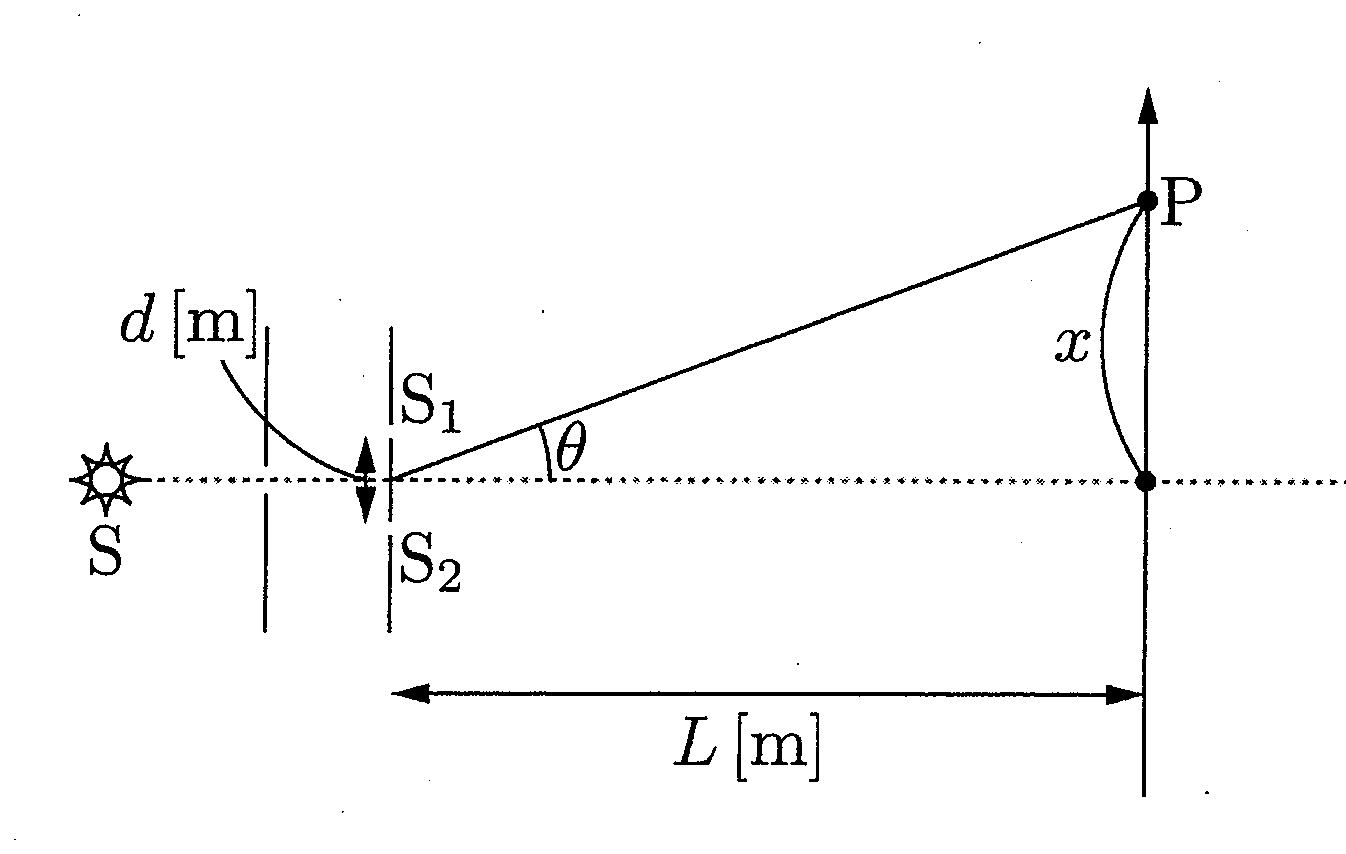
\includegraphics[keepaspectratio,width=68mm]{fig/ch25_a47_1.png}\end{center}
\ko{2} スクリーンはスリットから十分遠方にあるため，ガラス$\mathrm{G}$への光の入射角はほぼ(1)の$\theta$に等しく，またこれはほぼ0である．そのため，光はガラス$\mathrm{G}$に対してほぼ垂直に入射するとみなせる．
       \begin{center}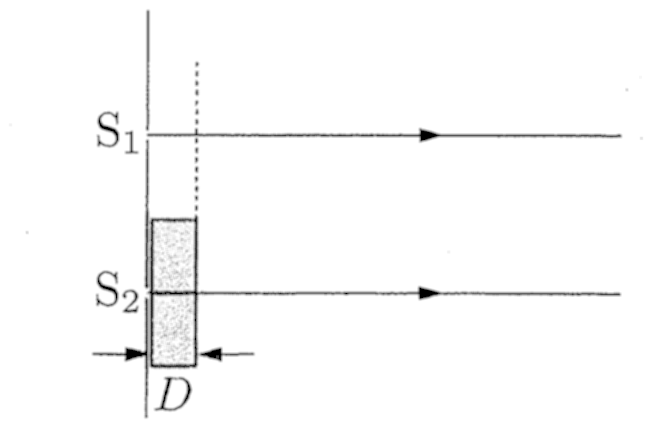
\includegraphics[keepaspectratio,width=46mm]{fig/ch25_a47_2.png}\end{center}
       \hspace{1zw}前図において，スリットから長さ$D\U{m}$の部分の光路長は，
       \[\mathrm{S_1}側：1\times D\U{m}\]
       \[\mathrm{S_2}側：n\times D\U{m}\]
       であるから，ガラス$\mathrm{G}$を置いたことにより，$\mathrm{S_2}$側を経由してくる光の方が光路長にして
       \[(n-1)D\U{m}\Ans\]
       だけ余分に通ってくることが分かる．
\ko{3} (1), (2)より，スクリーン上の$\mathrm{P}$点へは，$\mathrm{S_2}$を経由してくる光の光路の方が光路長にして
       \[d\frac{x}{L}+(n-1)D\U{m}\]
       だけ余分に通ってくることが分かる．よって，光路差が真空中の1波長の整数倍であれば強め合いとなるので，強め合うための条件は
       \[d\frac{x}{L}+(n-1)D=m\lambda\Ans\]
       \hspace{1zw}これより，$m$次の明線位置は，
       \[x_m=\frac{L}{d}\left\{m\lambda-(n-1)D\right\}\U{m}\]
       であり，明線は等間隔に出来ることが分かる．その間隔$\Delta x$は，
       \[\Delta x=x_{m+1}-x_m=\frac{L\lambda}{d}\U{m}\Ans\]
\end{komon}

\MonN{53}{回折格子}\par\nopagebreak
\begin{sisin}
$\mathrm{A}$問題と基本的には同じで，回折格子の干渉条件$d\sin\theta=m\lambda$を満たすような波長を求めればよい．単位を$\U{mm}$から$\U{m}$単位に直して考える点だけ注意しよう．

可視光とは$380\U{nm}$〜$780\U{nm}$の範囲の波長の光のことを言う．常識として覚えておくこと．
\end{sisin}
\KaiHead
\begin{komon}
\ko{1} 回折格子の干渉条件より，
       \[d\sin\theta=m\lambda\quad(ただし\,m\,は整数値)\]
       を満たすとき，$\mathrm{S}$の位置に明線が生じる．\hspace*{\fill}\Ans
\ko{2} この回折格子の格子定数は，
       \[d=\frac{1.0\times 10^{-3}}{250}=4.0\times 10^{-6}\U{m}\]
       であるから，$\mathrm{S}$の方向で強め合いとなる波長は
       \[\lambda=\frac{d\sin 30^\circ}{m}=\frac{2.0\times 10^{-6}}{m}\U{m}\]
       \[\hspace*{\fill}=\frac{2000}{m}\U{nm}\]
       である．これが可視光領域の$380\U{nm}$〜$780\U{nm}$の範囲に入るのは$m=3$, 4, 5のときで，
       \[\begin{aligned}
         \lambda=&6.7\times 10^2,\ 5.0\times 10^2,\\
                 &\hspace*{\fill}4.0\times 10^2\U{nm}\Ans
       \end{aligned}\]
\end{komon}

\Rank{C問題}
\MonN{54}{ロイドの鏡}\par\nopagebreak
\begin{sisin}
本問のように鏡を利用したヤングの実験には，本問のようなロイドの鏡と呼ばれる実験の他に，フレネルの合わせ鏡と呼ばれるものもあるが，いずれの場合にも，\underline{鏡によっ}\hskip0pt\underline{て反射す}\hskip0pt\underline{る光の経}\hskip0pt\underline{路を，鏡}\hskip0pt\underline{に対して}\hskip0pt\underline{折り返す}ことによってヤングの実験と同様な図に描き直すことができる．本問の場合，$\mathrm{S}$から出て$\mathrm{M}$で反射して$\mathrm{P}$に至る光の経路を，$\mathrm{M}$に対して折り返せば，スリット間隔$2d\U{m}$のヤングの実験になっていることが分かろう．ただし，\underline{鏡の反射}\hskip0pt\underline{の際に位}\hskip0pt\underline{相がずれる}ことを忘れないように．
\end{sisin}
\KaiHead
\begin{komon}
\ko{1} 点$\mathrm{P}$には，スリット$\mathrm{S}$から直接やってくる光と，いったん鏡$\mathrm{M}$によって反射してから$\mathrm{P}$にやってくる光の二つが重なり合って，干渉を起こす．
       \begin{center}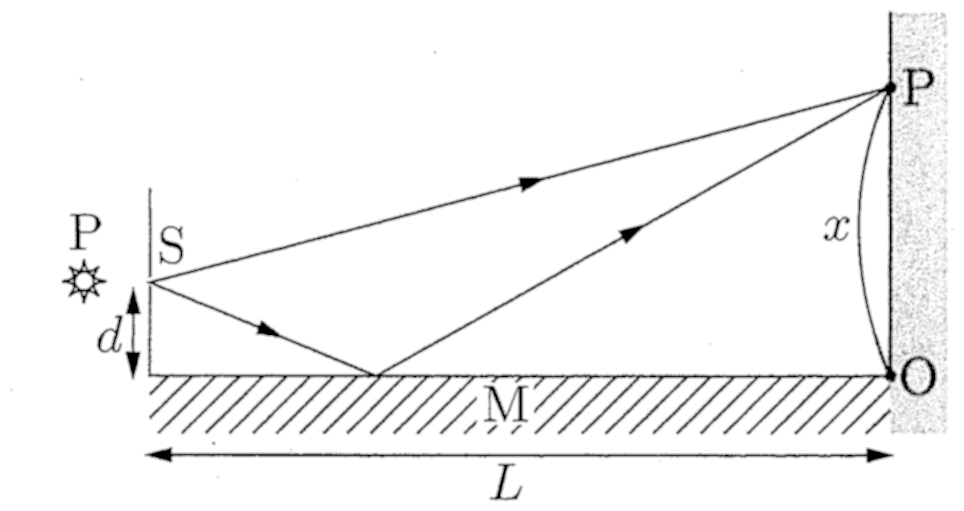
\includegraphics[keepaspectratio,width=68mm]{fig/ch25_a49_1.png}\end{center}
       \hspace*{\fill}\Ans
\ko{2} (1)の図において，$\mathrm{S}$から$\mathrm{M}$へ向かう光の経路を$\mathrm{M}$に対して折り返す．反射の法則より$\mathrm{S\to M}$の経路と$\mathrm{M\to P}$の経路は同じ傾きになっているので，$\mathrm{M}$に対して$\mathrm{S\to M}$の経路を折り返すとまっすぐな直線$\mathrm{S'P}$になる．
       \begin{center}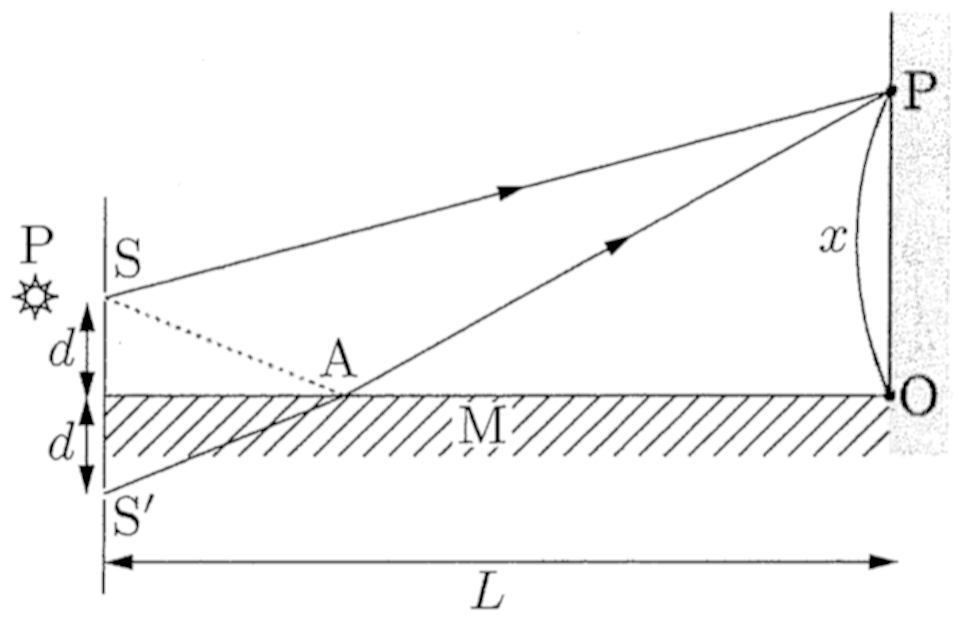
\includegraphics[keepaspectratio,width=68mm]{fig/ch25_a49_2.png}\end{center}
       \hspace{1zw}二つの光の経路差は，
       \[\begin{aligned}
         &(\overline{\mathrm{SA}}+\overline{\mathrm{AP}})-\overline{\mathrm{SP}}\\
         &\hspace{1zw}=(\overline{\mathrm{S'A}}+\overline{\mathrm{AP}})-\overline{\mathrm{SP}}\\
         &\hspace{1zw}=\overline{\mathrm{S'P}}-\overline{\mathrm{SP}}
       \end{aligned}\]
       であり，$\overline{\mathrm{S'P}}-\overline{\mathrm{SP}}$はスリット間隔が$2d\U{m}$のヤングの実験と同様にして求めることができるので，経路差は一次近似を用いて
       \[\overline{\mathrm{S'P}}-\overline{\mathrm{SP}}\fallingdotseq 2d\frac{x}{L}\U{m}\Ans\]
\ko{3} この光の二つの経路について，反射は$\mathrm{A}$点のみで起こっており，この反射は空気から鏡にぶつかっての反射であるから位相が$\pi$ずれる．よって，経路差によってさらに$\pi$のずれが生じるとき，すなわち経路差が1波長の整数倍＋半波長になっているときに$\mathrm{P}$点で二つの光が強め合う．よって強め合うのは，
       \[2d\frac{x}{L}=i\lambda+\frac{\lambda}{2}\quad(i\,は整数値)\]
       の条件が満たされるときである．これより，強め合う座標は，
       \[x=\frac{L\lambda}{4d}(2i+1)\quad(i\,は整数値)\]
       である．$x\geqq 0$であるから，$i$の取りうる値は
       \[i=0,\ 1,\ 2,\ \cdots\]
       であるから，この解を自然数$m\ (m\geqq 1)$を用いて表すと，
       \[x=\frac{L\lambda}{4d}(2m-1)\U{m}\Ans\]
       となる．

       \hspace{1zw}また，これより明線間隔$\Delta x$は，$m$を一つずらして差し引くことにより，
       \[\begin{aligned}
         \Delta x&=\frac{L\lambda}{4d}\left\{2(m+1)-1\right\}\\
                 &\hspace*{\fill}-\frac{L\lambda}{4d}(2m-1)\\
                 &=\frac{L\lambda}{2d}\U{m}\Ans
       \end{aligned}\]
       \begin{chuu}
       $i$と$m$の取り替えが分かりにくい人は，
       \[x=\frac{L\lambda}{4d}(2i+1)\]
       の解を書き下してみればよい．$x\geqq 0$で強め合いとなる位置は，
       \[x=\frac{L\lambda}{4d}\times 1\U{m}\]
       \[x=\frac{L\lambda}{4d}\times 3\U{m}\]
       \[x=\frac{L\lambda}{4d}\times 5\U{m}\]
       \[x=\frac{L\lambda}{4d}\times 7\U{m}\]
       \[\cdots(以下略)\]
       であり，これらをまとめて自然数$m$を用いて表すには，
       \[x=\frac{L\lambda}{4d}(2m-1)\U{m}\]
       と書けばよいことが分かる．
       \end{chuu}
\end{komon}

\MonN{55}{光速の測定実験（フーコーの実験）}\par\nopagebreak
\begin{sisin}
レーマーやブラッドリーは天体の観測を元に光速度を測定し，フーコーやフィゾーは鏡や歯車を利用することによって光速度を測定した．これらはいずれも原理は非常に単純で，物理の難しい特殊な知識が必要なわけではない．
\end{sisin}
\KaiHead
\begin{komon}
\ko{1} 光源$\mathrm{S}$から出た光が$\mathrm{M}$の向きへ反射するのは，回転鏡が$\dfrac{\pi}{4}\U{rad}$だけ傾いているときである．この状態から回転鏡が角度$\theta\U{rad}$だけ回転すると，戻ってきた光は入射角$\dfrac{\pi}{4}+\theta\U{rad}$で鏡$\mathrm{R}$に入射する．
       \begin{center}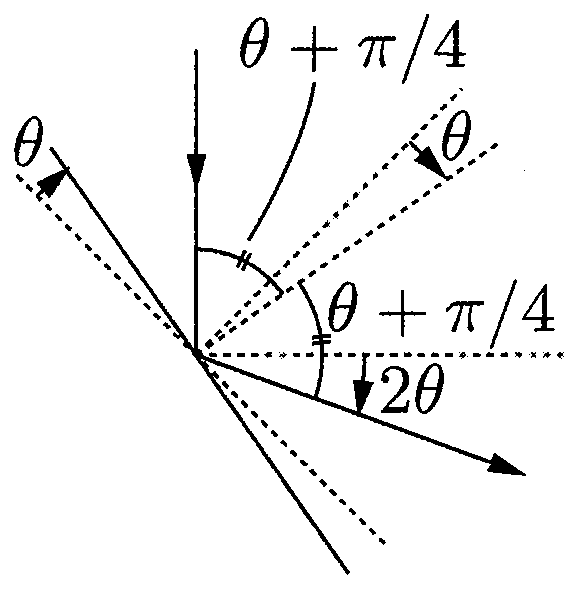
\includegraphics[keepaspectratio,width=44mm]{fig/ch25_a50_1.png}\end{center}
       \hspace{1zw}鏡$\mathrm{R}$では同じ角度$\dfrac{\pi}{4}+\theta\U{rad}$で反射していくので，入射角と反射角の開きは
       \[\left(\frac{\pi}{4}+\theta\right)\times 2=\frac{\pi}{2}+2\theta\U{rad}\]
       であるから，反射光は$\mathrm{RS}$の方向から下向きに角度$2\theta\U{rad}$だけ振れた向きになる．\hspace*{\fill}\Ans
\ko{2} $\mathrm{R}$の回転角速度は
       \[\omega=2\pi\times N\U{rad/s}\]
       であるから，角度$\theta\U{rad}$だけ回転するには
       \[t=\frac{\theta}{\omega}=\frac{\theta}{2\pi N}\U{s}\]
       の時間を要する．\hspace*{\fill}\Ans
\ko{3} 往復距離は$2l\U{m}$であるから，光が往復するのに要する時間は，
       \[t=\frac{2l}{c}\U{s}\Ans\]
\ko{4} (2)・(3)の答えが等しいので，
       \[c=\frac{4\pi Nl}{\theta}\U{m/s}\Ans\]
\ko{5} (4)の式に各値を代入して，
       \[\begin{aligned}
         c&=\frac{4\pi\times 800\times 20.0}{6.73\times 10^{-4}}\\
          &\fallingdotseq 2.99\times 10^{8}\U{m/s}\Ans
       \end{aligned}\]
\end{komon}

\MonN{56}{ヤングの実験}\par\nopagebreak
\begin{sisin}
まず経路差の式を導き，これを元にどの位置に明線が出来るかを求め，その間隔を求める．(3)では，式の中のどこを変更すればよいのかを考えて処理せよ．
\end{sisin}
\KaiHead
\begin{komon}
\ko{1} スクリーン上の座標$y\U{m}$の点$\mathrm{P}$について考える．直線$\mathrm{SP_0}$に対して，$\mathrm{AB}$の中点から$\mathrm{P}$点へ向けた角度を$\theta$とおく．
       \begin{center}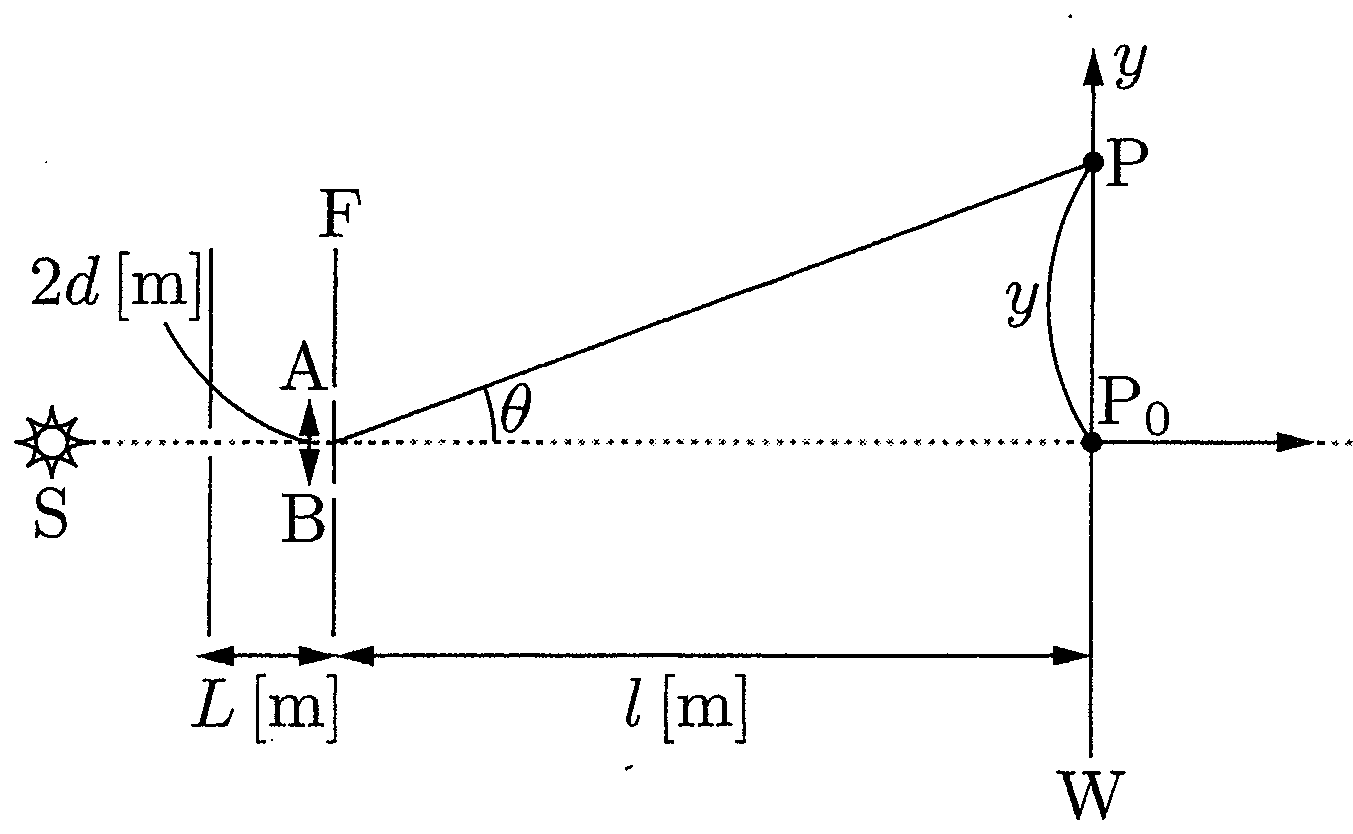
\includegraphics[keepaspectratio,width=68mm]{fig/ch25_a51_1.png}\end{center}
       \hspace{1zw}このとき，$\mathrm{A}$, $\mathrm{B}$から$\mathrm{P}$に向かう二つの光の経路差は，$|\theta|\ll 1$であることを利用して，
       \[\Delta D\fallingdotseq 2d\sin\theta\fallingdotseq 2d\tan\theta=2d\frac{y}{l}\U{m}\]
       と表される．単スリットから$\mathrm{A}$, $\mathrm{B}$までの距離が等しいので$\mathrm{A}$, $\mathrm{B}$は同位相の波源とみなせる．よって$\mathrm{P}$点で光が強め合うためには$m$を整数として，
       \[\Delta D\fallingdotseq 2d\frac{y}{l}=m\lambda\]
       であればよい．よってこれを解いて，$m$番目の明線の位置$y_m$は，
       \[y_m=m\frac{l\lambda}{2d}\U{m}\]
       である．この式と対応させると$\mathrm{P_0}$と$\mathrm{P_1}$はそれぞれ$m=0$, 1の場合に対応しているので，これより
       \[r=y_1-y_0=\frac{l\lambda}{2d}\U{m}\Ans\]
\ko{2} 最も明るい線$\mathrm{P_0}$は，もともと$\mathrm{A}$, $\mathrm{B}$から同一距離にあった点であるから，経路差が$0\U{m}$で強め合っている点である．単スリットを上方へ動かすと，単スリット$\mathrm{C}$から$\mathrm{B}$までの距離が，$\mathrm{C}$から$\mathrm{A}$までの距離に比べて長くなる（次図参照）．
       \begin{center}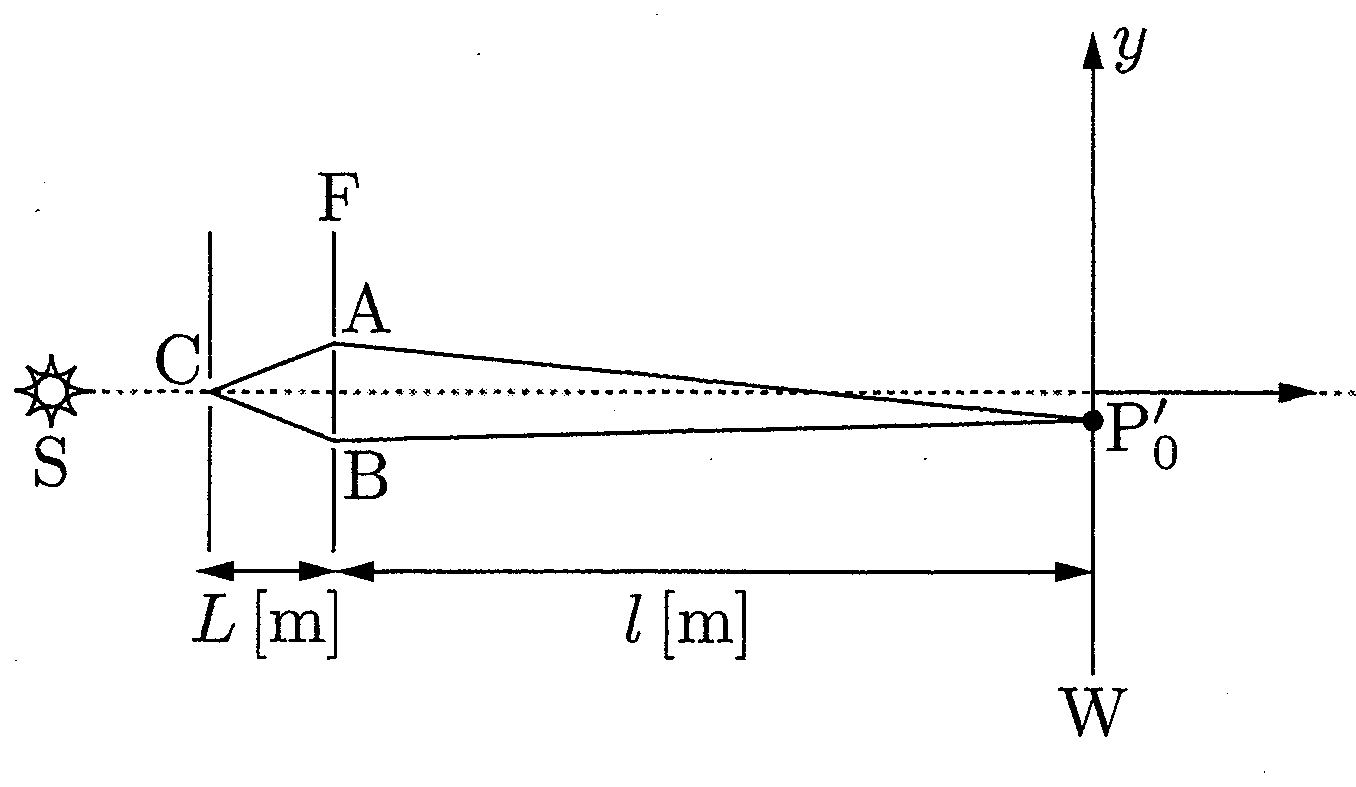
\includegraphics[keepaspectratio,width=68mm]{fig/ch25_a51_2.png}\end{center}
       \hspace{1zw}よって(2)の場合に経路差が0となる点を$\mathrm{P_0'}$とすると，$\overline{\mathrm{CA}}<\overline{\mathrm{CB}}$であるから$\overline{\mathrm{P_0'A}}>\overline{\mathrm{P_0'B}}$とならなければ経路差が0になることはない．

       \hspace{1zw}以上より，経路差$0\U{m}$で強め合う明線$\mathrm{P_0}$の位置は$-y$の向きに移動する．\hspace*{\fill}\Ans

       \hspace{1zw}またその負の向きへの移動距離を$\Delta y\U{m}\ (>0)$とすると，(1)と同様な一次近似より
       \[\overline{\mathrm{CB}}-\overline{\mathrm{CA}}\fallingdotseq 2d\frac{y_0}{L}\U{m}\]
       \[\overline{\mathrm{P_0'A}}-\overline{\mathrm{P_0'B}}\fallingdotseq 2d\frac{\Delta y}{l}\U{m}\]
       であるから，この二つの光の経路差は
       \[\begin{aligned}
         &\left(\overline{\mathrm{CA}}+\overline{\mathrm{P_0'A}}\right)-\left(\overline{\mathrm{CB}}+\overline{\mathrm{P_0'B}}\right)\\
         &\hspace{1zw}=2d\frac{\Delta y}{l}-2d\frac{y_0}{L}\U{m}
       \end{aligned}\]
       である．これが$0\U{m}$であるから，
       \[\frac{\Delta y}{l}-\frac{y_0}{L}=0\]
       \hspace{1zw}これを解いて，
       \[\Delta y=\frac{l}{L}y_0\U{m}\Ans\]
\ko{3} もともと$\mathrm{P_1}$点は，経路差が$\lambda\U{m}$となって強め合っていた点で，
       \[2d\frac{y_1}{l}=\lambda\]
       の強め合い条件を満たしていた点である．$\mathrm{F}$と$\mathrm{W}$の間隔を$l+x\U{m}$に延ばしたとき，経路差$\lambda\U{m}$の強め合いの点が$y_1+\Delta y_1$に移動したとすると，この点での強め合いの条件式は，
       \[2d\frac{y_1+\Delta y_1}{l+x}=\lambda\]
       である．$\mathrm{P_1}$点の強め合いの条件式と組み合わせると，
       \[\frac{y_1+\Delta y_1}{l+x}=\frac{y_1}{l}\]
       が成立するのでこれをまとめると，
       \[\Delta y_1=\frac{x}{l}y_1=\frac{xr}{l}\U{m}\]
       である．$\Delta y_1>0$であるから$\mathrm{P_1}$点は$+y$向きへと移動し，その移動距離は(1)の答えを代入して，
       \[\Delta y_1=\frac{xr}{l}=\frac{\lambda}{2d}x\U{m}\Ans\]
\end{komon}

\end{multicols}
